%==============================================================================
%  Application of Fourier Neural Operator as Autoregressive Neural Surrogate
%  for Geothermal Simulation
%
%  Springer Nature template (sn-jnl.cls v3.1, Dec 2024).
%  Author-year, Math & Physical Sciences reference style (sn-mathphys-ay).
%==============================================================================
\documentclass[pdflatex,sn-mathphys-ay]{sn-jnl}
%------------------------------- Packages -------------------------------------
% NOTE: sn-jnl already loads geometry, natbib (per the documentclass option),
% and hyperref internally -- do NOT load them here or LaTeX will clash.
% Fonts/encoding are handled by the class as well.

\usepackage{amsmath,amssymb,amsfonts,bm}
\usepackage{mathtools}
\usepackage{siunitx}              % \SI{640}{\meter}, units
\DeclareSIUnit{\darcy}{D}         % permeability: \si{\milli\darcy} -> mD
\usepackage{graphicx}
\usepackage{booktabs}             % \toprule \midrule \bottomrule
\usepackage{tabularx}             % full-width tables with ragged X column
\usepackage{array}
\usepackage{multirow}
\usepackage{xcolor}
\usepackage{tikz}
\usetikzlibrary{positioning,arrows.meta,fit,backgrounds,calc,shapes.misc,shapes.geometric}
\usepackage{algorithm}
\usepackage{algpseudocode}        % training-loop pseudocode
% cleveref must come after the class's hyperref (it does); drives all \cref's.
\usepackage[capitalize,noabbrev]{cleveref}
% The class ships uncolored links for submission. Uncomment for draft-time
% colored links:
% \hypersetup{colorlinks=true,allcolors=blue}

%---------------------------- Custom commands ---------------------------------
% Notation helpers -- adjust to taste.
\newcommand{\svec}{\mathbf{u}}            % reservoir state field
\newcommand{\action}{\mathbf{a}}           % well-control action
\newcommand{\model}{\mathcal{G}_\theta}    % learned operator
\newcommand{\R}{\mathbb{R}}
\newcommand{\fainttablerule}{\noalign{\vskip1pt{\color{black!20}\hrule height 0.03pt}\vskip1pt}}
\DeclareMathOperator{\diag}{diag}

% Editorial markers -- delete before submission.
\newcommand{\todo}[1]{\textcolor{red}{[\textbf{TODO:} #1]}}
\newcommand{\note}[1]{\textcolor{blue}{[\emph{#1}]}}

%---------------------- TikZ palette + styles (architecture fig) --------------
\definecolor{cGlobal}{HTML}{2C5F8A}   % global spectral branch
\definecolor{cLocal}{HTML}{2E7D5B}    % local patch branch
\definecolor{cHF}{HTML}{C25A1A}       % high-frequency branch
\definecolor{cCond}{HTML}{6A4C93}     % action / AdaLN conditioning
\definecolor{cAux}{HTML}{0F7B7B}      % auxiliary head
\definecolor{cLift}{HTML}{37474F}     % lifting / projection
\tikzset{
  >={Latex[length=2mm]},
  font=\footnotesize,
  io/.style={draw=none, font=\small\bfseries, text=black!80, align=center},
  blk/.style={rounded corners=2pt, draw=#1!70, fill=#1!10, text=black!85,
              line width=0.7pt, align=center, inner sep=4pt, minimum height=8mm},
  blk/.default=cLift,
  stack/.style={rounded corners=2pt, draw=cGlobal!70, fill=cGlobal!8,
                line width=0.7pt, align=center, inner sep=4pt},
  op/.style={circle, draw=black!70, fill=black!4, line width=0.7pt,
             inner sep=0pt, minimum size=5.5mm, font=\small},
  arr/.style={->, line width=0.7pt, draw=black!65},
  arrc/.style={->, line width=0.7pt, draw=cCond!75, densely dashed},
  zlabel/.style={font=\scriptsize\itshape, text=black!60},
  panel/.style={rounded corners=3pt, draw=black!45, densely dashed,
                line width=0.8pt, fill=black!2, inner sep=7pt},
  bgbox/.style={rounded corners=3pt, draw=black!20, fill=black!2,
                line width=0.6pt, inner sep=8pt},
}

%==============================================================================
\begin{document}

%------------------------------- Front matter ---------------------------------
\title[FNO Surrogate for Geothermal Simulation]{Application of Fourier Neural
       Operator as an Autoregressive Neural Surrogate for Geothermal Simulation}

\author*[1]{\fnm{Thanh} \sur{Nguyen}}\email{thanh2@ualberta.com}
\author[1]{\fnm{Juliana} \sur{Leung}}\email{juliana2@ualberta.ca}   % \todo{co-authors}

\affil*[1]{\orgdiv{Department of Civil \& Environmental Engineering}, \orgname{University of Alberta},
  \orgaddress{\city{Edmonton}}, \country{Canada}}

%------------------------------- Abstract -------------------------------------
\abstract{%
\todo{I don't like how this is right now. Will rewrite the abstract when everything is done}
Geothermal energy is a promising solution to the worldwide growing demand for
clean energy. Operating geothermal reservoirs requires careful engineering
decisions, often involving repeated numerical simulation runs to identify
optimal well controls. The expensive computational cost of these simulations has
motivated interest in data-driven surrogate models, where a neural network is
trained on simulation-generated data and acts as a proxy for future engineering
workflows. Building such neural surrogates is a challenging problem: we want the
model's predictions to closely match the simulator outputs, and to maintain that
accuracy autoregressively into the future, all while training on as little data
as possible. In this work, we propose two 3D geothermal datasets to evaluate our
surrogate model: one with homogeneous and one with heterogeneous porosity and
permeability fields. Training on only 300 trajectories, our adapted Fourier
Neural Operator with several architectural and training modifications achieves
\SI{0.1}{\percent} relative error on 3D pressure and temperature predictions, and
remains stable autoregressively across 156 time steps.
}

\keywords{geothermal reservoir simulation, Fourier neural operator,
  surrogate modeling, autoregressive rollout, operator learning}

\maketitle

%============================== 1. Introduction ================================
\section{Introduction}
\label{sec:intro}

Numerical simulators have long supported geothermal reservoir management tasks such as
history matching, well-placement and control optimization, uncertainty quantification, and
production forecasting. Common non-isothermal simulators include SHEMAT \citep{shemat},
FEFLOW \citep{feflow}, OpenGeoSys \citep{opengeosys}, ECLIPSE \citep{eclipse}, and CMG STARS
\citep{stars}. Although these tools employ different discretization strategies, they
generally rely on repeated linearization and the iterative solution of linear systems.
Consequently, their computational cost increases with spatial resolution, physical
complexity, and simulation duration. This cost is particularly prohibitive in iterative
engineering workflows such as optimal well control, where thousands of simulations may be
required to explore the decision space.

The high cost of repeated numerical simulations has motivated the development of neural
surrogate models as efficient approximations of high-fidelity reservoir dynamics. Neural
operators, including the Fourier Neural Operator (FNO) \citep{li2021fno}, are particularly
attractive because they learn mappings between function spaces and can predict spatiotemporal
pressure and temperature fields. Recent studies have demonstrated the potential of neural
operators trained on simulation-generated data. For example,
\citet{xueRobustPhysicsconstrainedNeural2026} employ a U-FNO-based architecture and construct
a dataset containing more than 9,000 three-dimensional reservoir simulations spanning a
20-year period. Their dataset varies reservoir depth, anisotropic permeability and porosity,
well controls, and other geological parameters. Rather than advancing the reservoir state
autoregressively, their model predicts the complete 20-year evolution of pressure and
temperature in a single forward pass.

Whole-horizon prediction is effective when the control schedule is known and fixed in
advance. However, many downstream applications require the surrogate to interact with a
dynamically changing control schedule. In reinforcement learning or model-predictive
control, for example, a policy may select new well controls after observing each predicted
reservoir state. An autoregressive surrogate is better suited to these settings because it
advances the reservoir state incrementally while conditioning each prediction on the latest
state and control action.

Accurate autoregressive prediction nevertheless introduces additional challenges. Because
each prediction becomes an input to the next prediction, small one-step errors can accumulate
and move the model away from the data distribution encountered during training, resulting in
unstable long-horizon rollouts. Moreover, deep neural networks, including FNOs, exhibit a
spectral bias toward learning low-frequency components before resolving higher-frequency
features. This behavior is particularly problematic for geothermal forecasting, where
localized phenomena such as thermal plumes and fronts are often characterized by
high-frequency, fine-scale features. Several methods have been proposed to improve autoregressive stability and the recovery of
high-frequency features. Pushforward training exposes a surrogate to its own predictions
during training, enabling it to learn how to correct the errors that arise during rollout.
PDE-Refiner uses noise injection and iterative denoising to model the autoregressive process
while emphasizing high-frequency features. Similarly, \citet{loglofno} achieves more stable autoregressive rollouts by proposing architectural
modifications that provide an explicit pathway for learning high-frequency features, together
with a radially binned spectral loss that penalizes errors in mid- and high-frequency
modes. The H1 loss has also been shown empirically to improve the recovery of high-frequency components by
penalizing errors in both field values and their spatial gradients.

Motivated by the need for efficient and stable autoregressive surrogates, this work makes
three primary contributions:
\begin{itemize}
  \item We extend the LOGLO-FNO architecture with adaptive layer normalization (AdaLN;
  \citep{adaln, film}) to improve its performance in well-control-conditioned geothermal
  pressure and temperature forecasting.
  \item We develop a training scheme that combines mean squared error, H1,
  material-balance, and radially binned spectral losses with pushforward training to
  improve the stability of autoregressive rollouts. We show that this scheme improves
  long-horizon performance not only for our proposed architecture but also for baselines
  including UNet, FNO, UFO, and U-FNO.
  \item We construct a dataset of heterogeneous geothermal reservoir simulations spanning a
  three-year period, with varying reservoir properties and well schedules. We demonstrate
  that reasonable performance can be achieved with very limited training data, as little as
  300 trajectory samples.
\end{itemize}


%=============================== 2. Dataset Generation and Learning Problem Formulation ===============
\section{Dataset Generation and Learning Problem Formulation}
\label{sec:data_and_learning}

In this section, we first describe the dataset used to train and evaluate our surrogate model and other baselines. 
Then we formulate the autoregressive prediction of pressure and temperature as predicting the residual between each timestep like in 
Euler discretization. 

\subsection{Dataset Generation}
We generate a heterogeneous dataset with 400 simulation trajectories, each trajectory
spans 156 weekly timesteps, corresponding to three years of operation. 
We use CMG STARS simulator and enable the dual-permeability (DUALPERM) setting, allowing every run to carry
separate matrix and fracture properties. The reservoir spans \SI{640}{\meter} in
width, \SI{320}{\meter} in length, and \SI{160}{\meter} in height, discretized
into $\SI{10}{\meter} \times \SI{10}{\meter} \times \SI{10}{\meter}$ cell blocks, giving
$64 \times 32 \times 16 = 32{,}768$ cells in total. The wells are arranged in an 
inverted five-spot pattern, with 2 injectors and 7 producers, as shown in
\cref{fig:well-pattern}. 

\begin{figure}[t]
  \centering
  \makebox[\textwidth]{%
    \begin{minipage}[b]{0.40\textwidth}
      \centering
      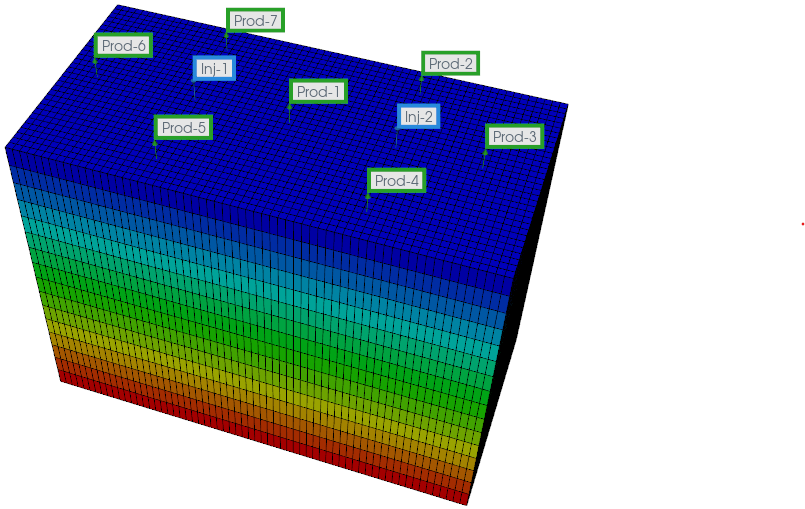
\includegraphics[width=\linewidth,trim=0 0 175bp 0,clip]
                      {figures/Figure2WellPatternA.png}\\[-0.2em]
      \textbf{(a)}
    \end{minipage}\hspace{0.01\textwidth}%
    \begin{minipage}[b]{0.68\textwidth}
      \centering
      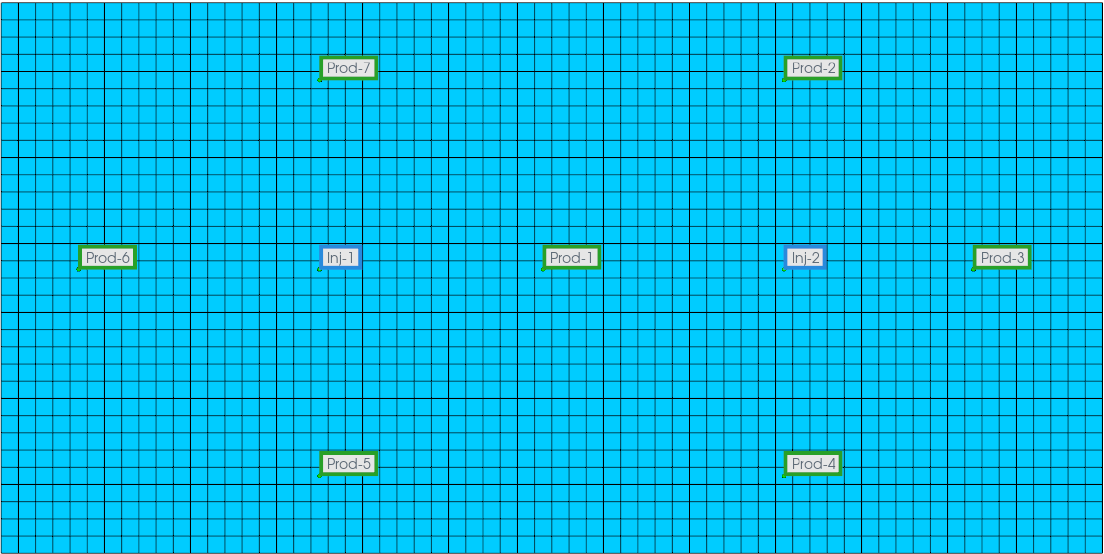
\includegraphics[width=\linewidth]{figures/Figure2WellPatternB.png}\\[-0.2em]
      \textbf{(b)}
    \end{minipage}}
  \caption{Reservoir domain and stacked inverted five-spot well pattern with
           two injectors and seven producers. \textbf{(a)} Three-dimensional
           view of the gridded reservoir domain. \textbf{(b)} Top-down view
           showing the well locations.}
  \label{fig:well-pattern}
\end{figure}

%-------------------- 3.1.1 Porosity, permeability ----------------------------
\subsubsection{Porosity, Permeability, and Other Simulation Parameters}
\label{sec:rock}
We want to create a reservoir with realistic properties. From the Ngatamariki geothermal field, Taupo Volcanic Zone, New Zealand, \cite{matrixTaupo}
presents matrix porosity ranging from 3\% to 20\%, and matrix permeability from \SI{0.00037}{\milli\darcy} to \SI{0.25}{\milli\darcy}, depending on whether the core
sample is pore-dominated or microfracture-dominated. Also in the Taupo Volcanic Zone, natural fractures in different rock types
can have permeability ranging from \SI{30}{\milli\darcy} to \SI{130}{\milli\darcy} \citep{fractureTaupo}. Inspired by the two studies, we generate our porosity and permeability realizations 
around these values. 

More specifically, we use unconditional Gaussian simulation with omnidirectional variograms
to generate 400 matrix porosity realizations and 400 fracture porosity realizations. The horizontal variogram is spherical with 10 lags of 
\SI{10}{\meter}, \SI{150}{\meter} search
radius, range \SI{100}{\meter}, nugget 0.1, and sill 0.9. The vertical variogram
is spherical with 5 lags of \SI{10}{\meter},
\SI{80}{\meter} search radius, range \SI{50}{\meter}, and same nugget and sill of 0.1 and 0.9 respectively. The variogram parameters are listed in \cref{tab:hetero-variogram}.
Matrix porosity is drawn with mean 0.05 and variance $2.5 \times 10^{-5}$, and
fracture porosity with mean 0.005 and variance $1 \times 10^{-6}$. To ensure
every block sustains some flow, we clip matrix porosity to $[0.035, 0.065]$ and
fracture porosity to $[0.002, 0.008]$, corresponding to $\pm 3$ standard
deviations about each mean.

Permeability is then derived from porosity. Matrix permeability follows
\begin{equation}
  k_{\text{matrix}} = \exp\!\left(29.182291\,\phi - 4.017112\right)\ \si{\milli\darcy},
  \label{eq:k-matrix}
\end{equation}
which keeps matrix permeability within $[0.05, 0.12]\ \si{\milli\darcy}$.
Fracture permeability follows a different formula
\begin{equation}
  k_{\text{fracture}} = \exp\!\left(3.21888 + 0.536479\,
    \frac{\phi - \mu_\phi}{\sigma_\phi}\right)\ \si{\milli\darcy},
  \label{eq:k-fracture}
\end{equation}
which keeps fracture permeability within $[5, 125]\ \si{\milli\darcy}$. These geological properties are summarized in \cref{tab:sim-props}. 

\begin{table}[t]
  \centering
  \caption{Variogram parameters used for heterogeneous porosity realizations.}
  \label{tab:hetero-variogram}
  \begin{tabular}{lcc}
    \toprule
    Parameter & Horizontal variogram & Vertical variogram \\
    \midrule
    Simulation type & \multicolumn{2}{c}{Unconditional Gaussian simulation} \\
    Variogram model & Spherical & Spherical \\
    Directionality & Omnidirectional & Omnidirectional \\
    Number of lags & 10 & 5 \\
    Lag spacing & \(\SI{10}{\meter}\) & \(\SI{10}{\meter}\) \\
    Search radius & \(\SI{150}{\meter}\) & \(\SI{80}{\meter}\) \\
    Range & \(\SI{100}{\meter}\) & \(\SI{50}{\meter}\) \\
    Nugget & 0.1 & 0.1 \\
    Sill & 0.9 & 0.9 \\
    \bottomrule
  \end{tabular}
\end{table}

\begin{table}[t]
  \centering
  \caption{Simulation properties.}
  \label{tab:sim-props}
  \small
  \setlength{\tabcolsep}{6pt}
  \renewcommand{\arraystretch}{1.35}
  \begin{tabularx}{\linewidth}{@{}l>{\raggedright\arraybackslash}X@{}}
    \toprule
    Property & Values \\
    \midrule
    Initial pressure & \SI{25}{\mega\pascal} \\
    \fainttablerule
    Initial temperature & \SI{170}{\celsius} \\
    \fainttablerule
    Fracture spacing & \SI{2}{\meter} \\
    \fainttablerule
    Matrix porosity & \(\phi_m\sim\mathcal{N}(0.05,\,2.5\times10^{-5})\), clipped \([0.035,0.065]\) \\
    \fainttablerule
    Fracture porosity & \(\phi_f\sim\mathcal{N}(0.005,\,1\times10^{-6})\), clipped \([0.002,0.008]\) \\
    \fainttablerule
    Matrix perm. & \(\begin{aligned}[t]
      k_m&=\exp(29.182291\phi_m-4.017112)\ \si{\milli\darcy},\\
      k_m&\in[0.05,0.12]\ \si{\milli\darcy}
    \end{aligned}\) \\
    \fainttablerule
    Fracture perm. & \(\begin{aligned}[t]
      z_f&=(\phi_f-\mu_{\phi})/\sigma_{\phi},\\
      k_f&=\exp(3.21888+0.536479z_f)\ \si{\milli\darcy},\\
      k_f&\in[5,125]\ \si{\milli\darcy}
    \end{aligned}\) \\
    \bottomrule
  \end{tabularx}
\end{table}



%-------------------- 2.1.2 Well control schedules ----------------------------
\subsubsection{Well Control Schedules}
\label{sec:schedules}

We want our surrogate model to be robust and able to capture highly irregular and
chaotic physical dynamics. With this goal in mind, we randomly divide the 156
timesteps into chunks of 2, 3, or 4 weeks. Within each chunk, we sample the rate
for each injector from a uniform distribution between \SI{500}{} and
\SI{3000}{\cubic\meter\per\day}. For the producers, we scale the sum of all
injector rates by a scalar drawn from a uniform distribution between 0.92 and
1.05, ensuring the producers do not draw the reservoir down too quickly, and then
randomly allocate this scaled total across the 7 producers. To make the dynamics
even more irregular, every injector and producer has a \SI{10}{\percent} chance of
shutting in during each chunk, where its rate is set to zero and the remaining
well rates are adjusted accordingly. This procedure yields highly irregular
well-control schedules, which in turn drive complex, chaotic reservoir dynamics to
test our surrogate model's ability to learn and generalize with limited data.


%--------------------------- 2.2 Learning Problem Formulation ----------------------------
\subsection{Learning Problem Formulation}
The goal for our surrogate modelis to learn to predict pressure and temperature fields at the next weekly timestep given the current pressure and temperature fields, well control, and geological properties. 
For simplicity, porosity and permeability realizations are assumed to be unchanged over time. We
define the state at time \(t\) as
\[
  \svec_t =
  [T_{\text{matrix}}(t), T_{\text{fracture}}(t),
   P_{\text{matrix}}(t), P_{\text{fracture}}(t)],
\]
where each component is represented on the \(64 \times 32 \times 16\)
three-dimensional grid described previously. The control signal (or action), \(\action_t\), is
defined on the same grid and contains two channels: the surface condition well-rate
constraint, replicated over perforation layers 3--12, and a binary shut-in
indicator, replicated over the same interval. The time-invariant geological
properties are denoted by
\(\phi=[\phi_{\text{matrix}},\phi_{\text{fracture}}]\) and
\(\kappa=[\kappa_{\text{matrix}},\kappa_{\text{fracture}}]\), representing the
matrix and fracture porosity and permeability fields, respectively. The
surrogate therefore approximates the one-step transition from
\((\svec_t,\action_t,\phi,\kappa)\) to \(\svec_{t+1}\).

This formulation assumes that the reservoir dynamics satisfy the Markov
property: prediction of \(\svec_{t+1}\) requires only the current state
\(\svec_t\) and current control \(\action_t\), rather than the complete preceding
trajectory. This assumption is consistent with the governing mass- and
energy-balance equations, which are first order in time and determine the
instantaneous state derivative from the present state and controls. The
numerical simulator used to generate the training data has the same structure,
advancing each time step by solving an implicit linear system assembled from
the current state and well controls. Consequently, no earlier states or actions
are required by the surrogate at the prediction point.

Because pressure and temperature vary smoothly between consecutive weekly time
steps, most of the reservoir state remains nearly unchanged even under
randomized well controls. We therefore parameterize the surrogate as a residual
update, analogous to an Euler discretization of the reservoir dynamics:
\begin{equation}
  \frac{\hat{\svec}_{t+1}-\svec_t}{\Delta t}
  =
  \model(\svec_t,\action_t,\phi,\kappa).
  \label{eq:euler}
\end{equation}
For the unit time step \(\Delta t=1\), the update becomes
\begin{equation}
  \hat{\svec}_{t+1}
  =
  \svec_t+\model(\svec_t,\action_t,\phi,\kappa).
  \label{eq:update}
\end{equation}
where \(\model\) learns the incremental state change induced by the reservoir
dynamics and well controls instead of reconstructing the comparatively large
background field at every step. 
%================================ 3. Methods ===================================
\section{Methods}
\label{sec:methods}

\subsection{Background on Fourier Neural Operator and LOGLO-FNO}
\label{sec:background_fno}
Much like how neural networks approximate functions, neural operators approximate operators, i.e,
mappings between function spaces 
$\mathcal{G}: \mathcal{A}\rightarrow\mathcal{U}$, where $\mathcal{A}$ and
$\mathcal{U}$ are Banach spaces defined on a bounded domain. Following
\cite{li2021fno}, a Fourier Neural Operator (FNO) represents this map with
three components: a lifting map $\mathcal{P}$ that embeds the input field into a
higher-dimensional latent space, a sequence of Fourier layers
$\{\mathcal{L}_{\ell}\}_{\ell=0}^{L-1}$, and a projection map $\mathcal{Q}$ that
returns the latent representation to the output dimension:
\begin{align}
z^{0} &= \mathcal{P}(a), &
z^{\ell+1} &= \mathcal{L}_{\ell}(z^{\ell}), &
u &= \mathcal{Q}(z^{L}).
\end{align}
Each Fourier layer transforms the latent field to Fourier space, applies
learnable weights to a retained set of modes, transforms the result back to
physical space, and combines the spectral update with a pointwise neural
network:
\begin{align}
\mathcal{L}_{\ell}(z)
&= \sigma\!\left(\mathcal{K}_{\ell}(z)+\mathrm{MLP}_{\ell}(z)\right), \\
\mathcal{K}_{\ell}(z)
&= \mathcal{F}^{-1}\!\left(
  \mathcal{W}_{\ell}\odot\mathcal{F}(z)
\right).
\end{align}
Here, $\mathcal{F}$ denotes the Fourier transform, $\mathcal{W}_{\ell}$ denotes
the learnable spectral weights for the retained modes in layer $\ell$,
$\mathrm{MLP}_{\ell}$ is a pointwise MLP, and $\sigma$ is a nonlinear activation.
This spectral convolution is not a full convolution in the sense of the
convolution theorem; it is a truncated convolution that retains only a selected
set of lower-frequency modes. The truncation allows FNOs to model large-scale
structure efficiently, but it also limits their ability to capture localized
high-frequency features.

FNOs and related variants have achieved strong performance on a wide variety of
operator-learning tasks, including earth atmosphere modeling \citep{fourcastnet3}, ocean
circulation prediction \citep{oceancirculation}, carbon storage digital twins 
\citep{carbonstorage}, and many others. 
However, the standard FNO
architecture can struggle when the solution requires localized high-frequency
detail because the spectral convolution explicitly truncates higher Fourier
modes. This limitation is important for turbulent flows such as high-Reynolds
number Navier-Stokes problems and for geothermal reservoir dynamics, where
irregular well controls interact with complex porosity and permeability
anisotropy. To increase high-frequency modeling capacity, the LOGLO-FNO
architecture~\citep{loglofno} augments the global FNO branch with local and
high-frequency branches. \cref{fig:loglo-fno} shows the internal structure of a
single LOGLO-FNO block.

\begin{figure}[t]
  \centering
  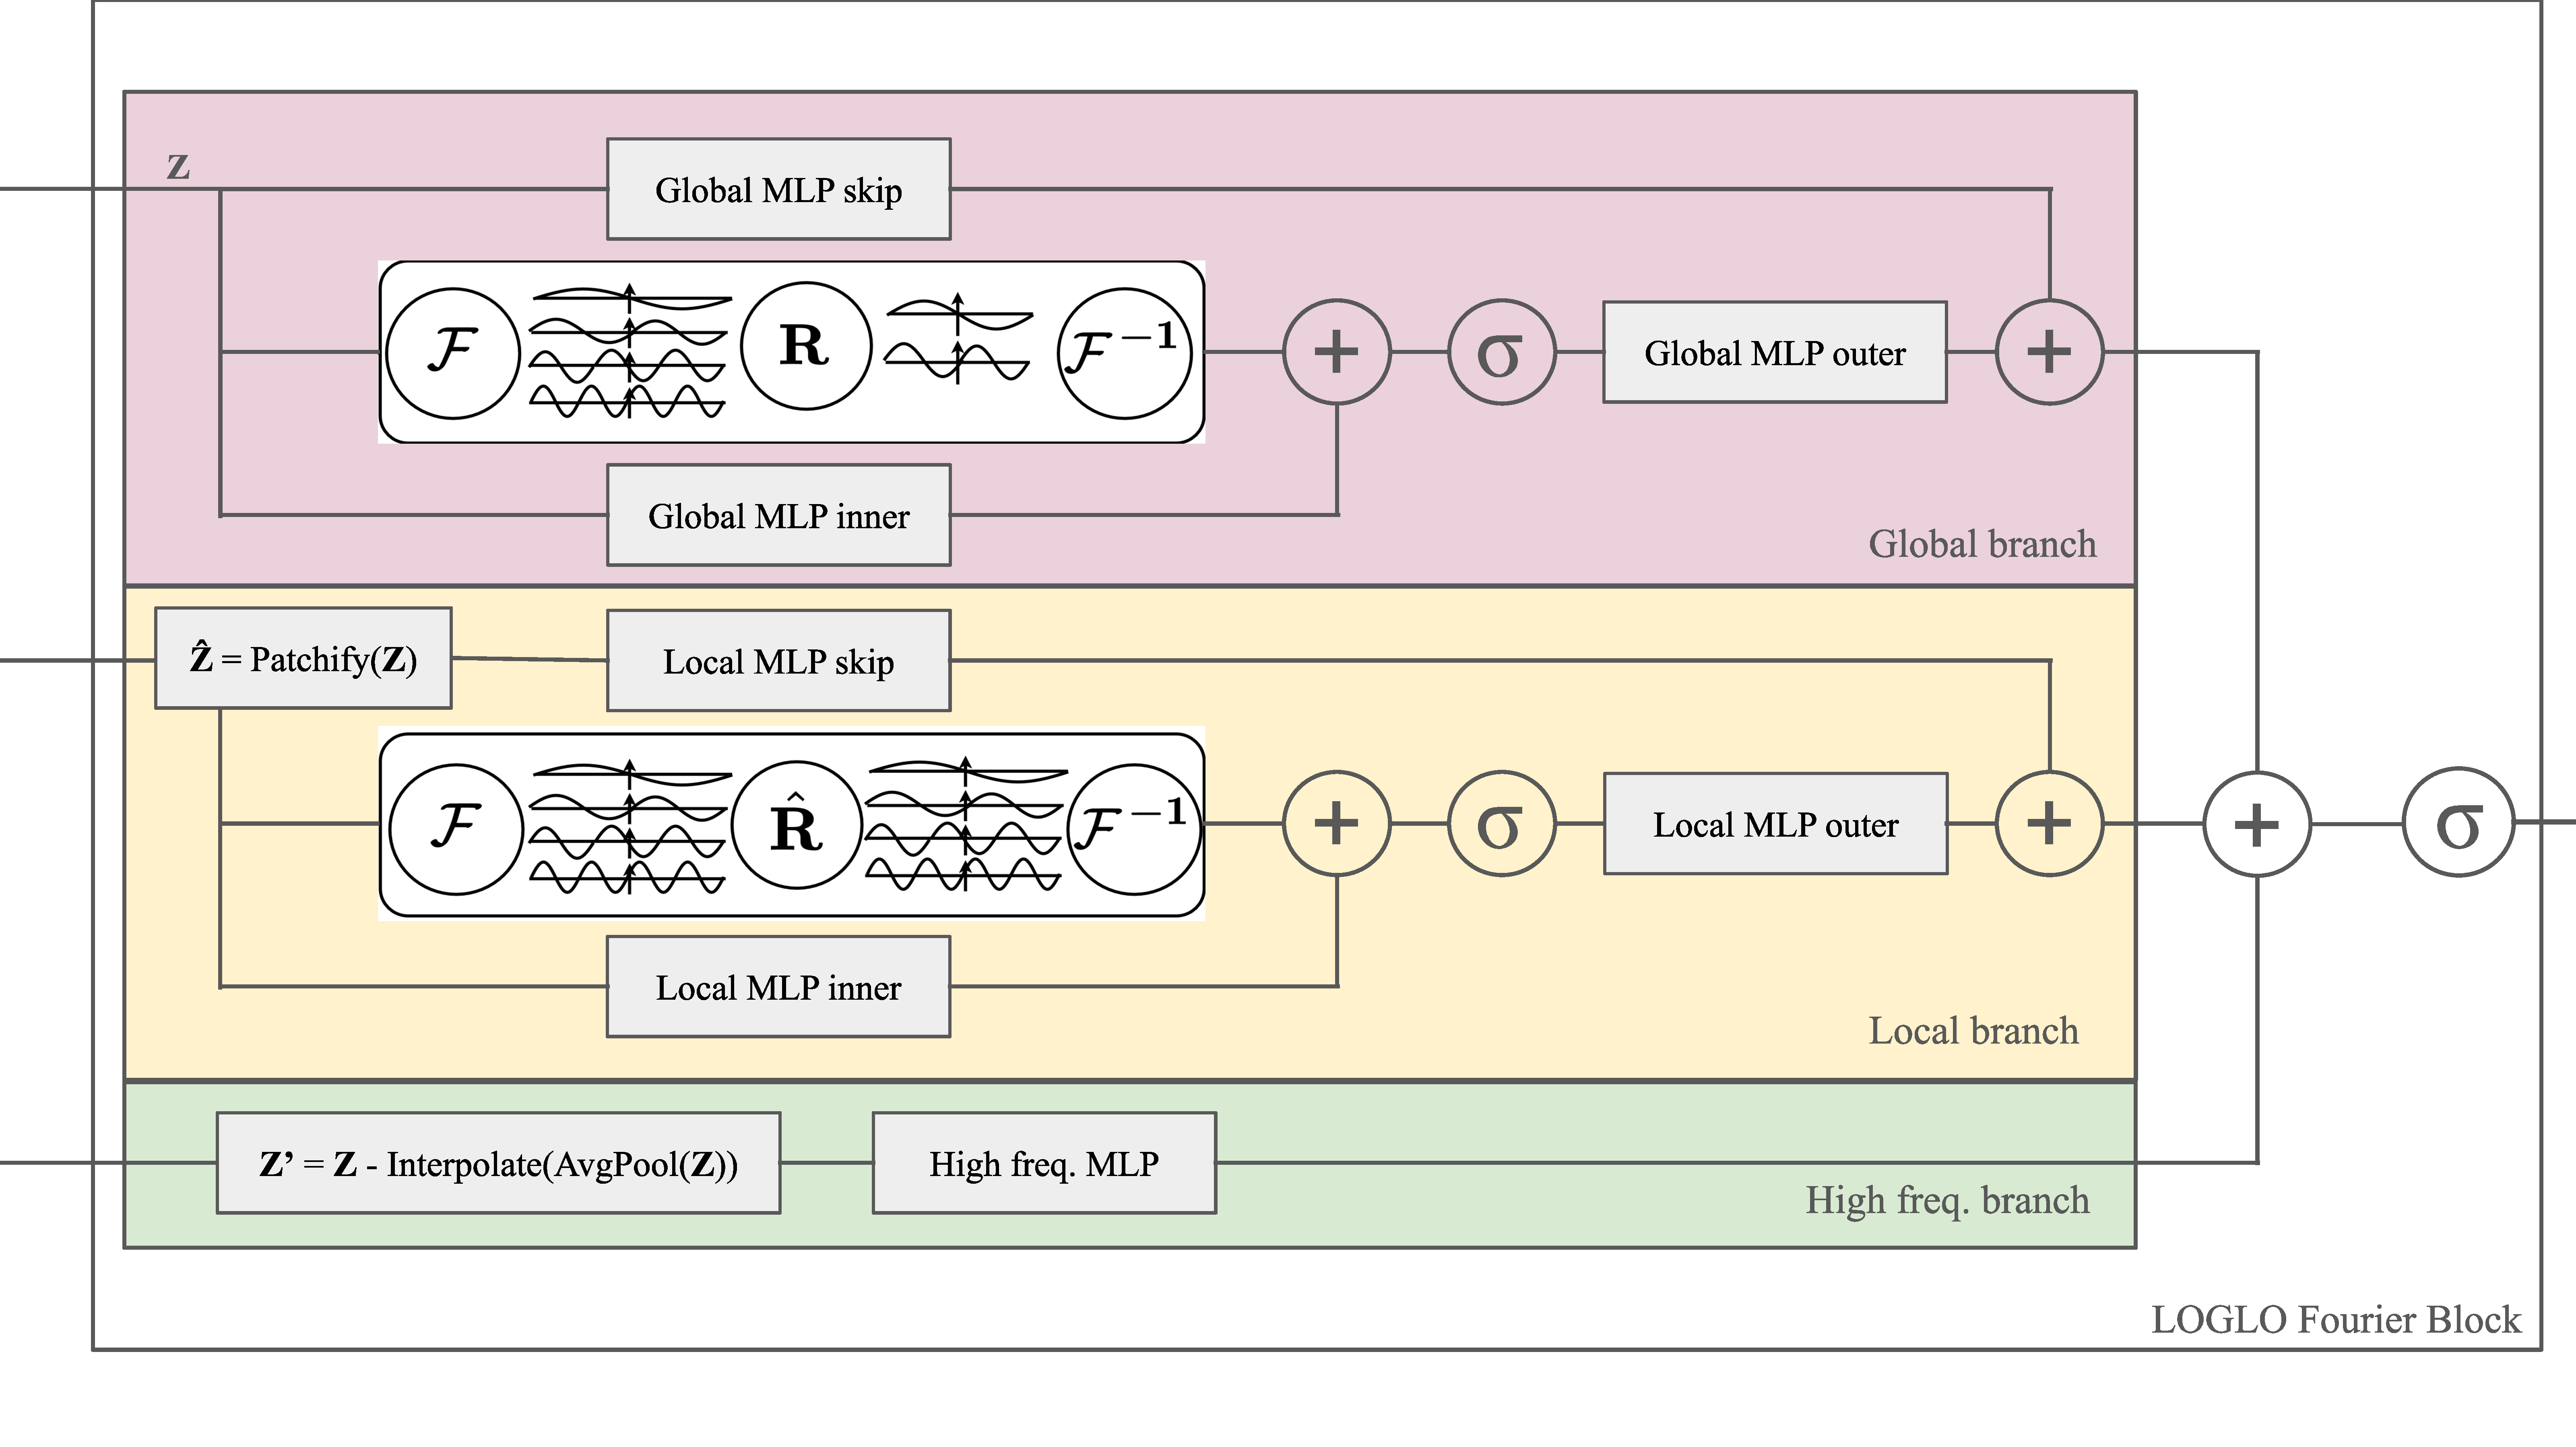
\includegraphics[width=\textwidth]{figures/vanilla_loglo.pdf}
  \caption{A single Fourier block in the LOGLO-FNO architecture, as documented in \cite{loglofno}.
  The three branches are color coded: global spectral in red, local patch in yellow, and high-frequency in green.}
  \label{fig:loglo-fno}
\end{figure}

More concretely, the global, local, and high-frequency branches are lifted
separately using three different lifting maps. Let $x$ denote the input field.
The initial latent fields are
\begin{align}
z^{(0)} &= \mathcal{P}_{glob}(x), &
\hat{z}^{(0)} &= \mathcal{P}_{loc}(x), &
z'^{(0)} &= \mathcal{P}_{hf}\!\left(\operatorname{HF}(x)\right),
\end{align}
where $\mathcal{P}_{glob}$, $\mathcal{P}_{loc}$, and $\mathcal{P}_{hf}$ are the
global, local, and high-frequency lifting maps, respectively.
Inside block $\ell$, the global branch (red in \cref{fig:loglo-fno}) closely
resembles a standard FNO block, with an additional outer MLP and skip MLP:
\begin{align}
\mathcal{L}_{glob}^{\ell}(z)
&= \mathrm{MLP}_{\mathrm{skip},glob}^{\ell}(z)
 + \mathrm{MLP}_{\mathrm{outer},glob}^{\ell}\!
   \left[
   \sigma\!\left(
     \mathcal{K}_{trunc}^{\ell}(z)
     + \mathrm{MLP}_{\mathrm{inner},glob}^{\ell}(z)
   \right)
   \right].
\end{align}

The local branch (yellow in \cref{fig:loglo-fno}) has the same block structure
as the global branch, but uses a different Fourier operator. Instead of applying
a truncated Fourier operator over the entire domain, we first divide the domain
into patches and then apply a Fourier operator that retains all modes within
each patch. This allows the local branch to capture localized high-frequency
features without the computational cost of a full-resolution Fourier operator
over the entire domain:
\begin{align}
  \hat{z} &= \operatorname{Patchify}(z),\\
  \mathcal{L}_{loc}^{\ell}(\hat{z})
  &= \mathrm{MLP}_{\mathrm{skip},loc}^{\ell}(\hat{z})
  + \mathrm{MLP}_{\mathrm{outer},loc}^{\ell}\!
    \left[
    \sigma\!\left(
      \mathcal{K}_{all}^{\ell}(\hat{z})
      + \mathrm{MLP}_{\mathrm{inner},loc}^{\ell}(\hat{z})
    \right)
    \right].
\end{align}

Finally, the high-frequency operator is defined as
\begin{equation}
z' = \operatorname{HF}(z)
= z-\operatorname{Interpolate}\!\left(\operatorname{AvgPool}(z)\right).
\end{equation}
It extracts high-frequency information by removing a low-frequency approximation
obtained through average pooling and interpolation. This high-frequency stream
is then processed by a pointwise MLP (green in \cref{fig:loglo-fno}) to capture
features that the local branch may miss.

The three branch outputs are fused by element-wise addition and passed through a
nonlinear activation before entering the next block. After the first block, the
local branch uses the fused latent representation, and the high-frequency
residual is recomputed from that same fused representation. Alongside the novel architecture,
\cite{loglofno} also propose a training loss called \emph{Radially Binned Spectral Loss}, where
we penalize mid- and high-frequency modes of the error between prediction and ground truth, 
in order to encourage
the model to sharpen fine details predictions. 
Together, they achieve an impressive improvement 
from 12\% to 40\% relative error reduction on multiple benchmarks 
compared to a standard FNO. In this work,
we adapt the LOGLO-FNO architecture to our 3D geothermal surrogate 
modeling task with new well control conditioning and 
training modifications that lead to stable autoregressive rollouts 
and strong performance with very limited training data. We describe these modificaitions
in detail in \cref{sec:arch}.





%---------------------------- 3.2 Problem formulation -------------------------
  \subsection{LOGLO-FNO Architecture with Adaptive Layer Normalization}
\label{sec:arch}

We adapt the LOGLO-FNO architecture to represent the residual transition
\(\model\). Its local--global decomposition is well suited to geothermal
reservoir dynamics, which combine field-scale transport with localized
well-induced responses. A straightforward implementation would concatenate the
four dynamic-state channels in \(\svec_t\), the two control channels in
\(\action_t\), and the four porosity and permeability channels into a single
10-channel LOGLO-FNO input. In our experiments, however, this configuration did
not provide the best performance (Table~\ref{tab:performance}). Instead, we use
a separate conditioning pathway to encode the well controls and static
porosity/permeability fields and to modulate the LOGLO-FNO blocks. This design
improves predictive performance and produces more stable autoregressive
rollouts. We hypothesize that separate conditioning is advantageous because the
controls and geological properties are not components of the evolving dynamic
state and can therefore be represented more effectively as modulators of the
state update. For the homogeneous dataset, porosity and permeability are
constant across all samples and are consequently omitted from the model inputs.

Specifically, the LOGLO-FNO blocks are conditioned through Adaptive Layer
Normalization (AdaLN), rather than by directly concatenating the conditioning
variables with the dynamic-state channels. Let
\(\mathbf{c}_t=[\action_t,\phi,\kappa]\) denote the conditioning tensor for the
heterogeneous case and \(\mathbf{c}_t=\action_t\) for the homogeneous case. The
modulation encoder is a lightweight CNN with the sequence
\[
  \text{MLP}
  \rightarrow \operatorname{GELU}
  \rightarrow \operatorname{Conv3D}_{3\times3\times3}
  \rightarrow \operatorname{GELU}
  \rightarrow \operatorname{Conv3D}_{3\times3\times3}
  \rightarrow \operatorname{GELU}
  \rightarrow \text{MLP},
\]
The pointwise MLP layers mix the
control and geological channels at each grid cell, whereas the two spatial
convolutions provide a small local receptive field. Consequently,
the encoder can learn spatially varying interactions between a well action and
the geological properties of its neighboring cells, thereby estimating how the
local reservoir response should modify the dynamic-state update. The encoder
maps these locally informed features to block-specific affine parameters:
\begin{equation}
  \{(\gamma^\ell,\beta^\ell)\}_{\ell=0}^{L-1}
  =
  \mathcal{E}_{\eta}(\mathbf{c}_t),
\end{equation}
where
\(\gamma^\ell,\beta^\ell\in\R^{C\times16\times64\times32}\) match the channel
and spatial dimensions of the hidden LOGLO-FNO representation. This
conditioning mechanism was first introduced by \cite{film} and gains popularity for providing
a robust way to condition vision transformer architectures for video and image generation.

Let \(z^{(\ell)}\), \(\hat{z}^{(\ell)}\), and \(z'^{(\ell)}\) denote,
respectively, the global, local, and high-frequency representations entering
block \(\ell\). AdaLN modulation is applied to the global and local pathways:
\begin{align}
  z_{\mathrm{mod}}^{(\ell)}
  &=
  (1+\gamma^\ell)\odot\operatorname{LayerNorm}(z^{(\ell)})
  +\beta^\ell,\\
  \hat{z}_{\mathrm{mod}}^{(\ell)}
  &=
  (1+\gamma^\ell)\odot\operatorname{LayerNorm}(\hat{z}^{(\ell)})
  +\beta^\ell.
\end{align}
The resulting global-branch output is
\begin{equation}
  g^{(\ell)}
  =
  \mathrm{MLP}_{\mathrm{outer},g}^{\ell}
  \left[
    \sigma\!\left(
      \mathcal{K}_{g}^{\ell}(z_{\mathrm{mod}}^{(\ell)})
      +
      \mathrm{MLP}_{\mathrm{inner},g}^{\ell}
      (z_{\mathrm{mod}}^{(\ell)})
    \right)
  \right]
  +
  \mathrm{MLP}_{\mathrm{skip},g}^{\ell}(z^{(\ell)}),
\end{equation}
and the local-branch output is computed analogously:
\begin{equation}
  l^{(\ell)}
  =
  \mathrm{MLP}_{\mathrm{outer},l}^{\ell}
  \left[
    \sigma\!\left(
      \mathcal{K}_{l}^{\ell}(\hat{z}_{\mathrm{mod}}^{(\ell)})
      +
      \mathrm{MLP}_{\mathrm{inner},l}^{\ell}
      (\hat{z}_{\mathrm{mod}}^{(\ell)})
    \right)
  \right]
  +
  \mathrm{MLP}_{\mathrm{skip},l}^{\ell}(\hat{z}^{(\ell)}).
\end{equation}

The high-frequency pathway is not modulated and is represented by a pointwise
MLP:
\begin{equation}
  h^{(\ell)}
  =
  \mathrm{MLP}_{\mathrm{hf}}^\ell(z'^{(\ell)}).
\end{equation}
This branch is intended to preserve high-frequency details of the dynamic state
without direct influence from the well controls or static geological fields.
Following the original LOGLO-FNO formulation described in
\cref{sec:background_fno}, the three branch outputs are combined as
\begin{equation}
  z^{(\ell+1)}
  =
  \sigma\!\left(
    g^{(\ell)}+l^{(\ell)}+h^{(\ell)}
  \right).
\end{equation}
After \(L\) blocks, the
output projection produces the residual state increment, yielding
\begin{equation}
  \hat{\svec}_{t+1}
  =
  \svec_t+\mathcal{P}_{\mathrm{out}}(z^L),
\end{equation}
where \(\mathcal{P}_{\mathrm{out}}\) denotes the output projection.

Many downstream applications require well-level quantities in addition to the
predicted pressure and temperature fields, including bottomhole pressure and
energy production rate. We therefore augment the surrogate with a lightweight
auxiliary prediction head. Rather than learning an additional dense spatial
field, this head exploits the known vertical-well geometry and extracts only the
state columns containing wells.

For each of the nine fixed well locations, the auxiliary head gathers the
complete vertical column from both the current state \(\svec_t\) and the
predicted next state \(\hat{\svec}_{t+1}\). Each column comprises all 16 depth
layers and four state channels; therefore, the input associated with each well
has dimension \(16\times4\times2\), where the final factor corresponds to the
current and predicted states. A shared per-well MLP embeds each column. The nine
resulting well embeddings are then concatenated and passed through a final
linear layer to obtain the auxiliary target vector:
\begin{equation}
  \mathbf{q}_t
  =
  \mathcal{H}_\psi(\svec_t,\hat{\svec}_{t+1})
  =
  \mathcal{H}_\psi\!\left(
    \svec_t,
    \svec_t+\model(\svec_t,\action_t,\phi,\kappa)
  \right).
  \label{eq:aux}
\end{equation}
In this study, \(\mathbf{q}_t\) contains the bottomhole pressures at all nine
wells and the energy production rates at the seven producer wells, for a total
of 16 scalar outputs. Because the diagnostic information for vertical wells is
concentrated along their columns, this architecture avoids predicting a dense
three-dimensional diagnostic field, reduces VRAM requirements, and can still
be trained jointly with the surrogate state predictor.



%---------------------------- 3.3 Model architecture --------------------------

\begin{figure}[tb]
  \centering
  % Bleed symmetrically into both margins: image is wider than \textwidth but
  % the surrounding \makebox keeps the caption at normal text width.
  \makebox[\textwidth]{%
    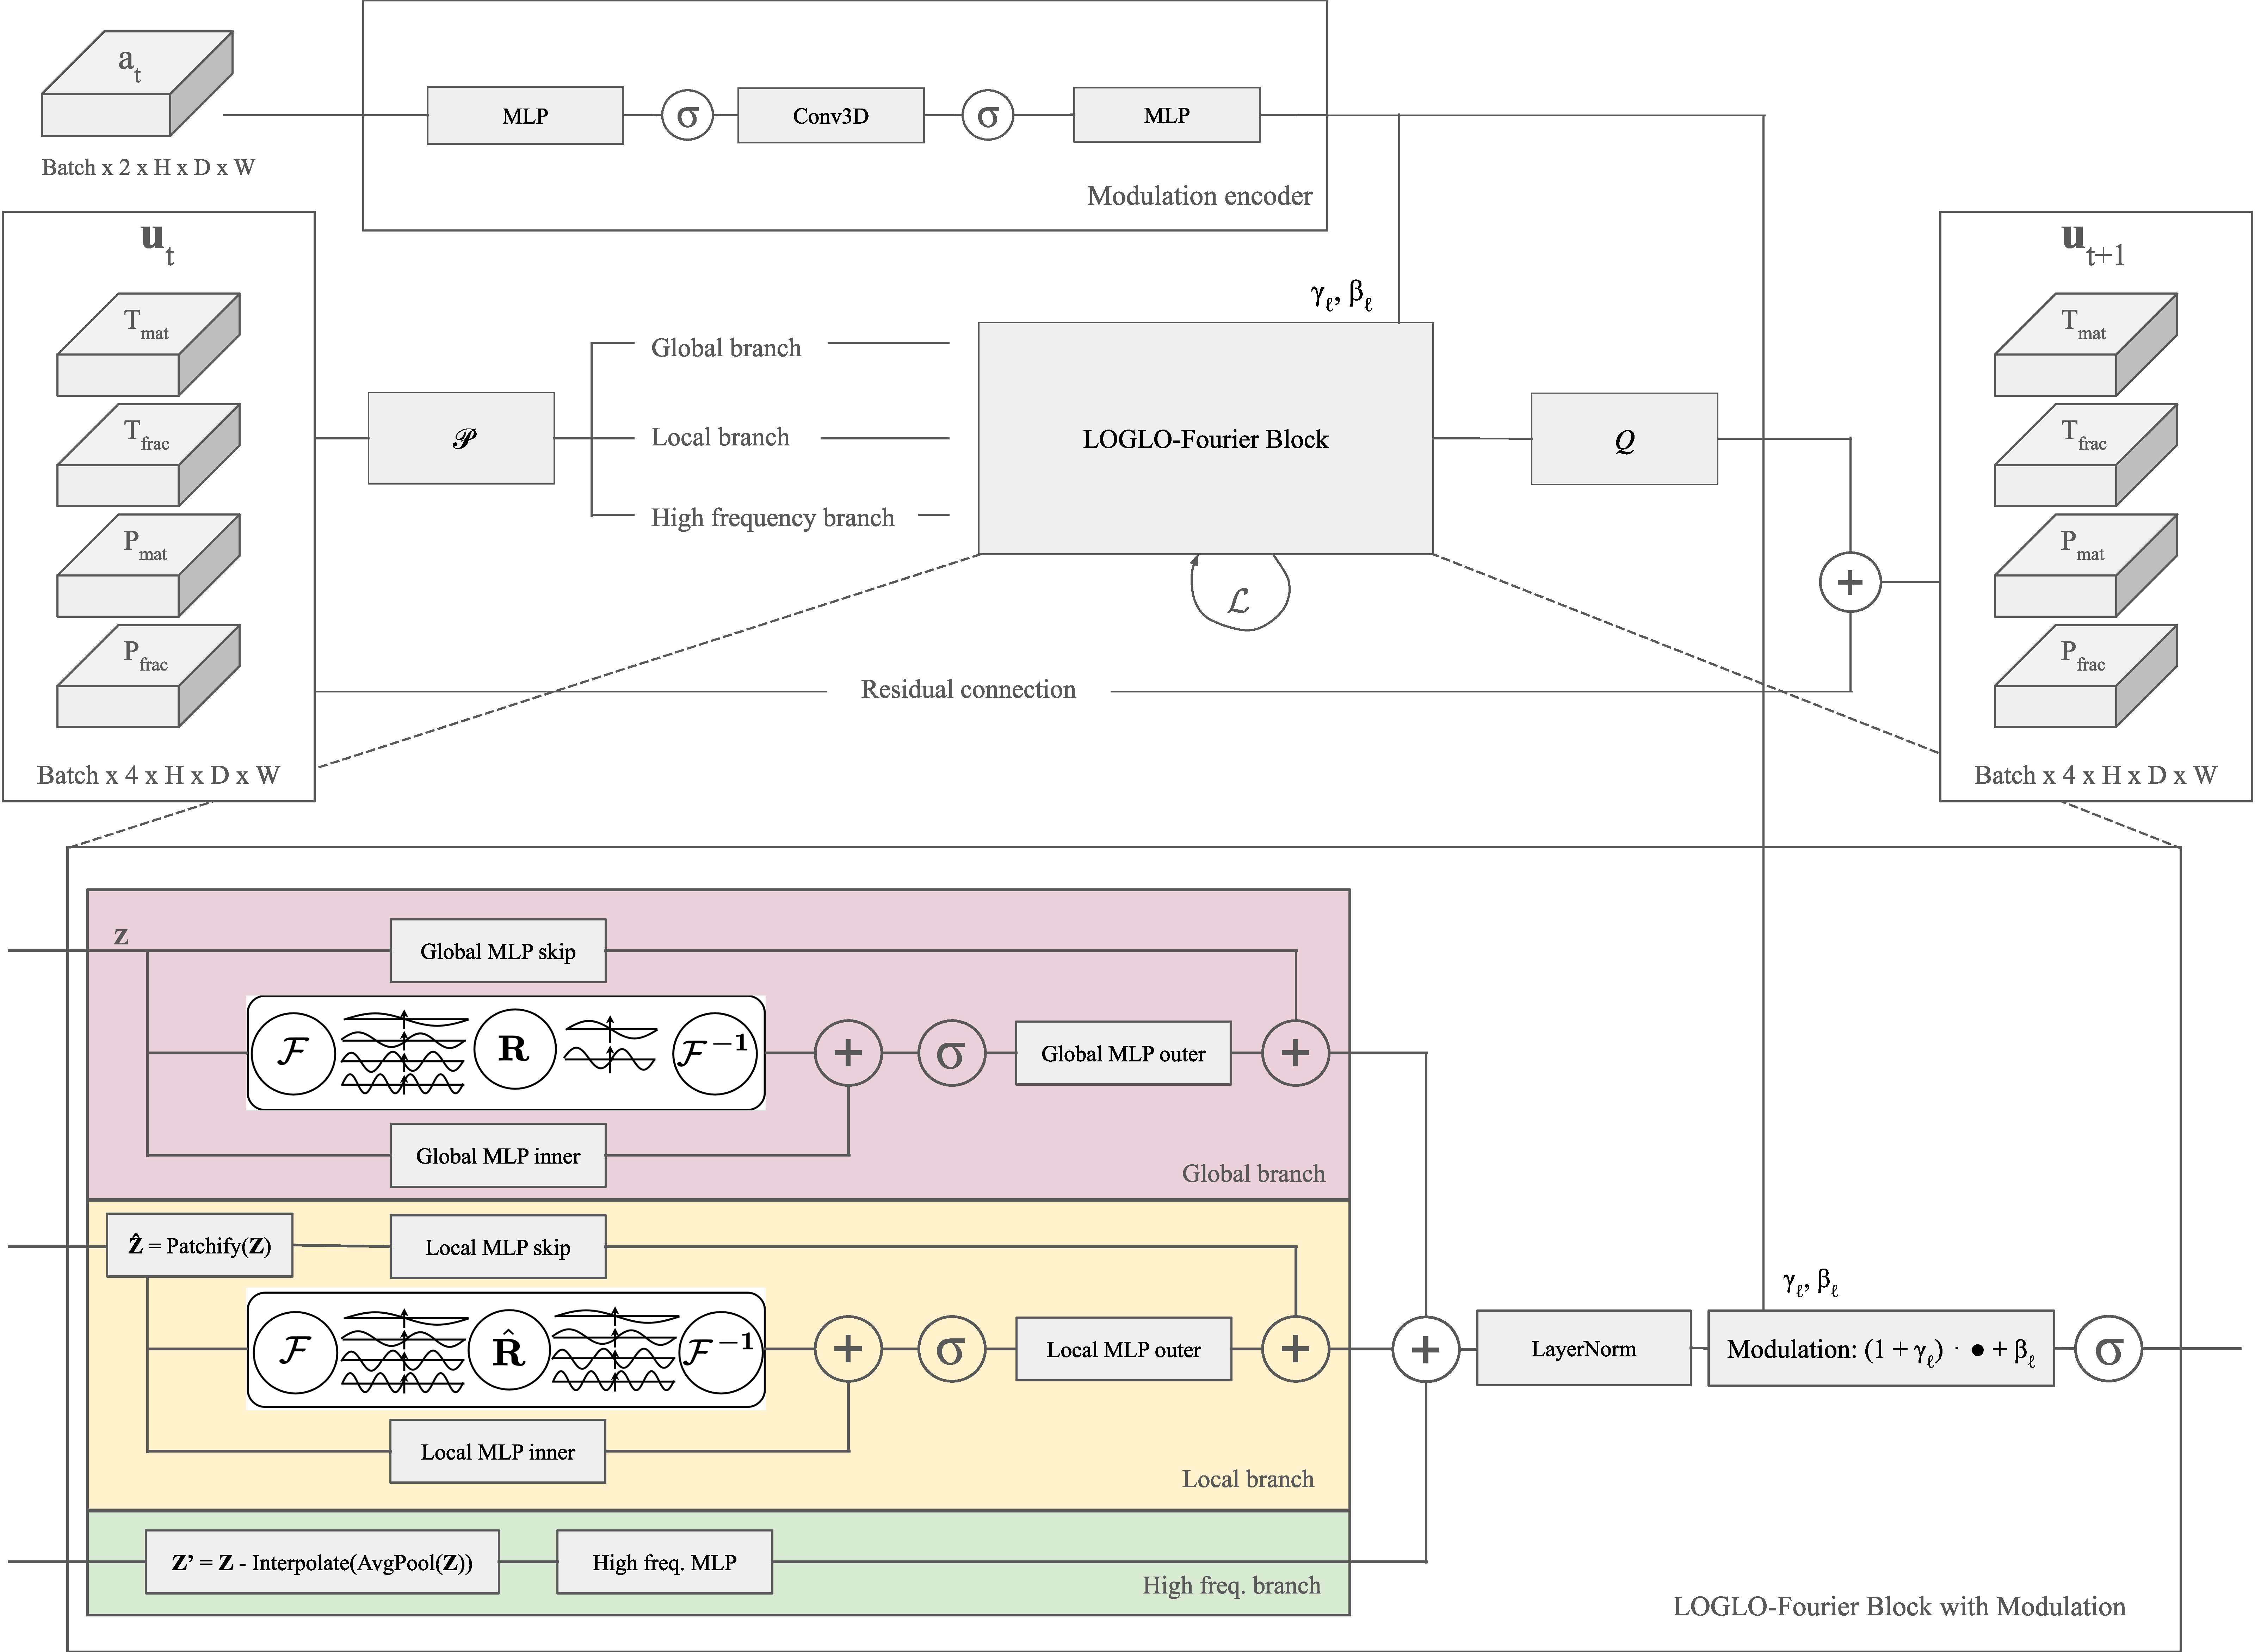
\includegraphics[width=\dimexpr\textwidth+1.6in\relax]{figures/loglofno_architecture.pdf}}
  \caption{\todo{Placeholder. Need new figure here}}
  \label{fig:arch}
\end{figure}

%---------------------------- 3.4 Training ------------------------------------
\subsection{Loss Functions}
The training objective is designed to make the predicted pressure and temperature
fields match the values produced by the numerical simulator as closely as
possible. We begin with mean squared error (MSE), since it directly penalizes
pointwise disagreement between the predicted next state
\(\hat{\svec}_{t+1}\) and the simulator state \(\svec_{t+1}\). In our
implementation, the two pressure channels receive twice the weight
of the two temperature channels since pressure is more sensitive to well controls. 
This choice reflects the larger sensitivity of
the pressure fields to well controls and the importance of matching pressure
accurately near injectors and producers.

MSE alone is not sufficient for this problem. Because it averages squared error
over the full three-dimensional domain, it tends to reduce the dominant
low-frequency error first. In other words, a model can obtain a low MSE by
capturing the broad spatial trend while still smoothing out sharper local
features. This is undesirable for geothermal simulation because several
important structures are high-frequency or localized: pressure changes near
wells, thermal fronts, and sharp contrasts induced by the well schedule. To
directly penalize these errors, we include the radially binned spectral loss used
in LOGLO-FNO~\citep{loglofno}. The residual
\(\hat{\svec}_{t+1}-\svec_{t+1}\) is transformed to Fourier space, its power is
grouped into radial frequency bins, and the loss is computed from the middle and
high frequency bands. We penalize mid- and high-frequency errors directly since the low
frequency components are already handled by the MSE term.

In addition to MSE and radial spectral loss, we use \(H^1\) Sobolev loss. This term
penalizes not only differences in the field values but also differences in their
spatial derivatives. Specifically, we calculate the finite difference
gradients in the \(x\), \(y\), and \(z\) directions for both the predicted and true fields,
then compute the mean squared error of these gradients. \cite{} show that H1 loss
further reduces the spectral bias towards low-frequency of neural networks by weighting
the high-frequency components more. Coincidentally, this loss also has a physical 
interpretation in our setting: the finite-difference flux
calculations depend on spatial pressure and temperature differences between neighbouring cells,
and by penalizing the gradient error, we encourage the model to respect 
the fluxes between cells.

On top of H1 loss that encourages the model to respect the local fluxes,
we further include a material balance equation (MBE) loss. The purpose of this
term is not to replace the simulator equations, but to provide a coarse physical
constraint that connects the predicted state change to the well-control action.
For a given transition from \(\svec_t\) to \(\hat{\svec}_{t+1}\), we compute an
approximate accumulation term from the predicted pressure and temperature change.
Pressure and temperature are first de-normalized, and fluid density is evaluated
using a simple compressibility and thermal-expansion model. We then compare this
accumulation with the source/sink term implied by the injection and production
rates. In normalized form,
\begin{equation}
  \mathcal{L}_{\mathrm{MBE}}
  =
  \mathbb{E}\!\left[
    \left(
      \frac{
        A(\svec_t,\hat{\svec}_{t+1}) - Q(\action_t)
      }{M_0}
    \right)^2
  \right],
  \label{eq:mbe-loss}
\end{equation}
where \(A\) is the predicted fluid-mass accumulation, \(Q\) is the net mass
introduced by the well controls over the step, and \(M_0=10^7\) is a
characteristic mass used to scale the loss to a reasonable range less
than one. This loss encourages the network to
learn a coupled relationship between well rates and the resulting pressure and
temperature changes, rather than treating the action as an arbitrary input
feature.

During early experiments, we also observed that the predicted pressure fields
could have the correct qualitative structure while still being shifted by a
small global offset. For example, the high-pressure regions around injectors and
the broader pressure trends were visible, but the mean pressure level over the
domain was slightly too high or too low. To target this specific error mode, we
add a mean-field pressure loss,
\begin{equation}
  \mathcal{L}_{\mathrm{meanP}}
  =
  \left\|
    \langle \hat{\svec}_{t+1}^{P} \rangle
    -
    \langle \svec_{t+1}^{P} \rangle
  \right\|_2^2,
  \label{eq:mean-pressure-loss}
\end{equation}
where \(\langle \cdot \rangle\) denotes a spatial average and the superscript
\(P\) denotes the two pressure channels. We apply this term only to pressure,
because the temperature fields did not show the same global-offset behavior.

Finally, we train the auxiliary head jointly with the state predictor. The
auxiliary head receives the current state \(\svec_t\) and the predicted next
state \(\hat{\svec}_{t+1}\), extracts the columns at the well locations, and
predicts 16 scalar quantities: 7 energy production rates and 9 bottomhole
pressures. We use a standard MSE loss for these auxiliary quantities. This is
sufficient in our experiments, likely because these outputs are low-dimensional
well-level quantities rather than full spatial fields.

Combining these terms, the one-step loss is
\begin{equation}
\begin{aligned}
  \mathcal{L}_{\mathrm{step}}
  ={}&
  3.0\,\mathcal{L}_{\mathrm{mse}}^{\mathbf{w}}
  + 0.5\,\mathcal{L}_{H^1}^{\mathbf{w}}
  + 3.0\,\mathcal{L}_{\mathrm{spec}}
  + \mathcal{L}_{\mathrm{MBE}}  \\
  &+ 2.0\,\mathcal{L}_{\mathrm{meanP}}
  + 0.1\,\mathcal{L}_{\mathrm{aux}} .
\end{aligned}
\label{eq:step-loss}
\end{equation}
The same loss weights are used for the homogeneous and heterogeneous
experiments, and for all baseline models. We summarize the purpose of each loss term
in \cref{tab:loss-purpose}. The loss weights were chosen empirically to balance the
different terms, and we find our model is not sensitive to small changes in these weights.

\begin{table}[t]
  \centering
  \caption{Purpose of each loss function used in the training objective.}
  \label{tab:loss-purpose}
  \begin{tabular}{@{}lp{0.68\textwidth}@{}}
    \toprule
    Loss function & Purpose \\
    \midrule
    MSE, \(\mathcal{L}_{\mathrm{mse}}\) & Pointwise error, low-frequency general trend \\
    \(H^1\) Sobolev loss, \(\mathcal{L}_{H^1}\) & Reduce low-frequency bias, encourage correct fluxes\\
    Radial spectral loss, \(\mathcal{L}_{\mathrm{spec}}\) & Mid to high-frequency error, enhance sharp fronts \\
    Material balance eqn. loss, \(\mathcal{L}_{\mathrm{MBE}}\) & Loose physical constraint \\
    Mean-field pressure loss, \(\mathcal{L}_{\mathrm{meanP}}\) & Prevent global pressure drifting\\
    Auxiliary-head MSE, \(\mathcal{L}_{\mathrm{aux}}\) & Predict well-level bottom-hole pressures and energy rates\\
    \bottomrule
  \end{tabular}
\end{table}


\subsection{Stabilizing Autoregressive Rollout with Pushforward Loss}
For each time step, the model predicts the next state from the current state and
the current well controls. Even if this one-step prediction is accurate, it will
still contain some error. Let this error be
\(\epsilon_t=\hat{\svec}_{t+1}-\svec_{t+1}\). During autoregressive rollout,
the next model input is not the simulator state \(\svec_{t+1}\), but the model
prediction \(\hat{\svec}_{t+1}\). As a result, the model is repeatedly evaluated
on slightly biased inputs. These small errors can accumulate over many steps and
eventually move the trajectory away from the distribution seen during ordinary
one-step training.

The key idea is therefore to train the model to recover from biased states. Ideally,
 we would like the model to produce an accurate next state even when
the input is \(\svec_t+\epsilon_t\) rather than the exact simulator state
\(\svec_t\). We approximate this situation using two complementary mechanisms:
adaptive Gaussian noise and a pushforward loss.

The first mechanism is adaptive input noise. With probability 0.8, we perturb the
current state before making the direct one-step prediction. The perturbation is
scaled by the spatial standard deviation of each state channel, so the noise
magnitude adapts to the local scale of each sample and variable:
\begin{equation}
  \tilde{\svec}_{t,c}
  =
  \svec_{t,c}
  +
  \alpha_c\,\sigma_{t,c}\,\epsilon_{t,c},
  \qquad
  \epsilon_{t,c}\sim\mathcal{N}(0,I),
  \label{eq:adaptive-noise}
\end{equation}
where \(\sigma_{t,c}\) is the spatial standard deviation of channel \(c\), and
\(\alpha=(0.0025,0.0025,0.025,0.025)\) for the two temperature and two pressure
channels, respectively. The target remains the clean simulator state
\(\svec_{t+1}\). Thus, the model learns to map a slightly perturbed current
state back to the correct next state instead of only learning from exact
simulator states.

The second mechanism is the pushforward loss~\citep{brandstetter2022pushforward}.
Instead of injecting a synthetic perturbation, pushforward training estimates the
kind of bias the model actually creates during autoregressive inference. We do
this by rolling the current model forward for several previous time steps without
gradient tracking. At training step \(g\), we define the maximum rollout length
available to the curriculum as
\begin{equation}
  K(g)=\min\!\left(10,\ 1+\left\lfloor \frac{g}{5000}\right\rfloor\right),
  \label{eq:k-curriculum}
\end{equation}
and sample \(k\) uniformly from \(\{1,\ldots,K(g)\}\). Starting from the
simulator state \(\svec_{t-k}\), we apply the model autoregressively through the
historical actions \(\action_{t-k},\ldots,\action_{t-1}\). This produces a
model-generated estimate of the current state, denoted
\(\hat{\svec}_t^{\mathrm{pf}}\). Since this state is obtained by feeding the
model its own outputs, it contains a realistic estimate of rollout drift.

After this no-gradient rollout, we make one gradient-tracked prediction from
\(\hat{\svec}_t^{\mathrm{pf}}\) using the current action \(\action_t\), and
compare the result with the simulator target \(\svec_{t+1}\). The pushforward
loss uses the same components as the direct one-step loss in
\cref{eq:step-loss}. Therefore, the model is not only asked to predict
\(\svec_{t+1}\) from the exact state \(\svec_t\), but also to predict
\(\svec_{t+1}\) from a state that resembles what it will see during
autoregressive inference. The total loss is
\begin{equation}
  \mathcal{L}_{\mathrm{total}}
  =
  \mathcal{L}_{\mathrm{step}}
  +
  \mathcal{L}_{\mathrm{pf}} .
  \label{eq:total-loss}
\end{equation}
For samples near the beginning of a trajectory where the requested history does
not exist, the pushforward term is masked out. The curriculum makes the task
progressively harder: early in training, the model only needs to recover from
short rollout errors, while later it is trained to recover from drift accumulated
over as many as 10 previous autoregressive steps.

\begin{algorithm}[t]
  \caption{One training step with adaptive noise and pushforward loss}
  \label{alg:training}
  \begin{algorithmic}[1]
    \Require Batch containing \(\svec_t,\svec_{t+1},\action_t\), history
             \(\{\svec_{t-k},\action_{t-k},\ldots,\action_{t-1}\}\), static porosity fields \(\phi\)
             and permeability fields \(\kappa\),
             and auxiliary target
             \(\mathbf{q}_{t+1}\)
    \State \(K \gets \min(10,1+\lfloor g/5000 \rfloor)\)
    \State Sample \(k \sim \mathrm{Uniform}\{1,\ldots,K\}\)
    \If{adaptive-noise draw succeeds}
      \State \(\tilde{\svec}_t \gets \svec_t + \alpha\,\sigma_t\,\epsilon\)
    \Else
      \State \(\tilde{\svec}_t \gets \svec_t\)
    \EndIf
    \State \(\hat{\svec}_{t+1} \gets \model(\tilde{\svec}_t,\action_t, \phi, \kappa)\)
    \State \(\widehat{\mathbf{q}}_{t+1}\gets \mathcal{H}_\psi(\svec_t,\hat{\svec}_{t+1})\)
    \State Compute \(\mathcal{L}_{\mathrm{step}}\) from \cref{eq:step-loss}
    \If{the sample has at least \(k\) previous states}
      \State \(\hat{\svec}^{(0)}\gets\svec_{t-k}\)
      \For{\(i=0,\ldots,k-1\)}
        \State \(\hat{\svec}^{(i+1)}
          \gets \model(\hat{\svec}^{(i)},\action_{t-k+i})\) \Comment{no gradients}
      \EndFor
      \State \(\hat{\svec}_{t+1}^{\mathrm{pf}}
        \gets \model(\hat{\svec}^{(k)},\action_t)\)
      \State Compute \(\mathcal{L}_{\mathrm{pf}}\) using the same terms as
             \(\mathcal{L}_{\mathrm{step}}\)
    \Else
      \State \(\mathcal{L}_{\mathrm{pf}}\gets 0\)
    \EndIf
    \State Update model parameters with
           \(\mathcal{L}_{\mathrm{step}}+\mathcal{L}_{\mathrm{pf}}\)
  \end{algorithmic}
\end{algorithm}

%============================== 4. Experiments =================================
\section{Experiments}
\label{sec:experiments}

\subsection{Experimental Setup}
\label{sec:setup}
While the primary objective is to assess our model's ability to generalize to geological realizations unseen during training, we also benchmark the proposed architecture against baseline models in both homogeneous and heterogeneous settings. This comparison aims to determine whether the incorporation of well schedule and geological property modulation improves the model's capacity to learn reservoir dynamics broadly, and more specifically, its ability to capture interactions arising from heterogeneous porosity and permeability distributions.
We train and evaluate all models on the homogeneous and heterogeneous datasets
described in \cref{sec:data}. Each dataset contains 400 simulated trajectories,
with 156 weekly timesteps per trajectory. Following the split used throughout
this study, 300 trajectories are used for training and 100 trajectories are held
out for testing. The same split is used for both the homogeneous and
heterogeneous datasets.

All inputs and targets are normalized before training. Temperature is min--max
normalized using the fixed range \([20,185]\ ^\circ\mathrm{C}\), and well rates
are normalized by the maximum rate of \(5000\) $\mathrm{m}^3/\mathrm{day}$. 
Pressure is also min--max
normalized, with dataset-specific ranges: \([1900,68000]\) $\mathrm{kPa}$ for the homogeneous
dataset and \([1300,70000]\) $\mathrm{kPa}$ for the heterogeneous dataset. 
For the heterogeneous
case, the static porosity and permeability fields are normalized using the
ranges used to generate the dataset (\cref{tab:sim-props}). The auxiliary targets are normalized
separately: bottomhole pressure uses the same pressure normalization as the state
fields, while energy production rate is normalized with a \(\log(1+x)\)
transform.

All models are optimized with AdamW \cite{} using batch size 4,
weight decay \(10^{-4}\), and an initial learning rate of \(8\times 10^{-4}\).
Each model is trained for 3000 epochs. The learning rate is warmed up linearly
for 4500 optimizer steps and then follows a cosine decay schedule to a minimum
learning rate of \(3\times 10^{-4}\). With 300 training trajectories and batch
size 4, this corresponds to 75 optimizer steps per epoch and 225000 optimizer
steps in total, so the warmup covers approximately 2\% of training. Gradients
are clipped before each optimizer step, with architecture-specific thresholds:
1.0 for FNO and Transolver as they are more sensitive to gradient instabilities, 
and 8.0 for UNet and LOGLO-FNO.

We maintain an exponential moving average (EMA) \citep{} of both the backbone model and
the auxiliary head, and use the EMA weights for validation and final
autoregressive evaluation. The EMA decay is 0.9995, corresponding to a half-life
of \(\log(0.5)/\log(0.9995)\approx 1386\) optimizer steps. This provides a
smoothed version of the learned parameters and reduces the effect of abrupt
updates late in training.

All experiments are run on 3/8th of an NVIDIA H100 GPU with 96 GB of VRAM provided
by the Digital Research Alliance of Canada.

\subsection{Baselines}
\label{sec:baselines}
We compare our well schedule and geological property modulated LOGLO-FNO against strong and 
relevant structrured-grid surrogate baselines. Specifically, we include 4 base FNO 3D models,
implemented using the \texttt{neuralop} library, with varying spectral modes and hidden widths to 
assess the effect of these architectural choices. We further more include 2 UNet3D models with different depths.
Additionally, we include two Transolver models, which leverage the latest transformer architecture, with varying
number of slices and hidden widths. Last but not least, we evaluate our model against a vanilla LOGLO-FNO model
to isolate the effect of our proposed modifications. A summary of the model configurations is provided 
in \cref{tab:baselines-models}. In terms of parameter counts, all baselines are bigger than 
our proposed LOGLO-FNO model, except for FNO modes [4, 16, 8] and hidden width 64, and Transolver
hidden width 128 and slice number 64.

\begin{table}[t]
  \centering
  \caption{Model configurations used in the experiment matrix. Each row is run
           for both the homogeneous and heterogeneous datasets. \emph{Params}
           are trainable backbone parameters for the homogeneous configuration
           (auxiliary head excluded), counted with \texttt{torchinfo}. LOGLO-FNO
           is included for context as the proposed model, not as a baseline.}
  \label{tab:baselines-models}
  \small
  \setlength{\tabcolsep}{4pt}
  \renewcommand{\arraystretch}{1.1}
  \begin{tabularx}{\linewidth}{@{}l l r >{\raggedright\arraybackslash}X@{}}
    \toprule
    Model & Family & Params & Configuration \\
    \midrule
    FNO m4x16x8 h64 & FNO & 11.9M & modes $[4,16,8]$, 5 layers, $h{=}64$ \\
    FNO m4x16x8 h128 & FNO & 47.6M & modes $[4,16,8]$, 5 layers, $h{=}128$ \\
    FNO m8x32x16 h64 & FNO & 66.1M & modes $[8,32,16]$, 4 layers, $h{=}64$ \\
    UNet3D d3 & UNet3D & 22.4M & depth 3, base $h{=}64$ \\
    UNet3D d4 & UNet3D & 90.3M & depth 4, base $h{=}64$ \\
    Transolver h128 s64 & Transolver & 7.8M & 8 layers, $h{=}128$, 8 heads, 64 slices \\
    Transolver h256 s32 & Transolver & 31.2M & 8 layers, $h{=}256$, 8 heads, 32 slices \\
    \addlinespace[2pt]
    \midrule[0.2pt]
    \addlinespace[2pt]
    Vanilla LOGLO-FNO & LOGLO-FNO & 13.8M & 5 blocks, $h{=}64$, no modulation \\
    Modulated LOGLO-FNO~(ours) & LOGLO-FNO & 14.1M & 5 blocks, $h{=}64$, modulation \\
    \bottomrule
  \end{tabularx}
\end{table}

\subsection{Evaluation Metrics}
\label{sec:metrics}
\todo{Relative $L_2$ / per-channel relative error, rollout error vs.\ horizon,
spectral error, auxiliary (BHP, energy rate) error.}

%================================ 5. Results ===================================
\section{Results}
\label{sec:results}

\subsection{Homogeneous Reservoir}
\label{sec:results-homo}
\todo{quantitative table + rollout-error-vs-time plot + qualitative fields.}

\begin{table}[t]
  \centering
  \caption{Test-set accuracy on the homogeneous dataset (lower is better).}
  \label{tab:results-homo}
  \begin{tabular}{lcccc}
    \toprule
    Model & Rel. $L_2$ (\%) & 156-step Rel. $L_2$ (\%) & Aux. error & Params \\
    \midrule
    UNet3D     & & & & \\
    FNO        & & & & \\
    Transolver & & & & \\
    LOGLO-FNO (ours) & & & & \\
    \bottomrule
  \end{tabular}
\end{table}

\subsection{Heterogeneous Reservoir}
\label{sec:results-hetero}
\todo{same structure as homogeneous; emphasize generalization across static
fields.}

\subsection{Ablations}
\label{sec:ablations}
\todo{pushforward on/off, individual loss terms, EMA, noise injection,
local-global branches.}

%================================ 6. Discussion ================================
\section{Discussion}
\label{sec:discussion}
\todo{Interpretation, failure modes, limitations (data regime, single reservoir
geometry), and implications for well-control optimization.}

%================================ 7. Conclusion ================================
\section{Conclusion}
\label{sec:conclusion}
\todo{Summarize contributions and outline future work.}

%---------------------------- Back matter -------------------------------------
\backmatter

\bmhead{Acknowledgements}
\todo{funding, compute (DRAC/Fir cluster), collaborators.}

\section*{Declarations}
\begin{itemize}
  \item Funding: \todo{}
  \item Competing interests: \todo{}
  \item Data availability: \todo{links to datasets}
  \item Code availability: \todo{link to repository}
\end{itemize}

% The bibliography style is selected by the documentclass option
% (sn-mathphys-ay) -- do not use \bibliographystyle here.
\bibliography{references}

\end{document}
